\begin{figure*}
\begin{subfigure}{0.34\textwidth}
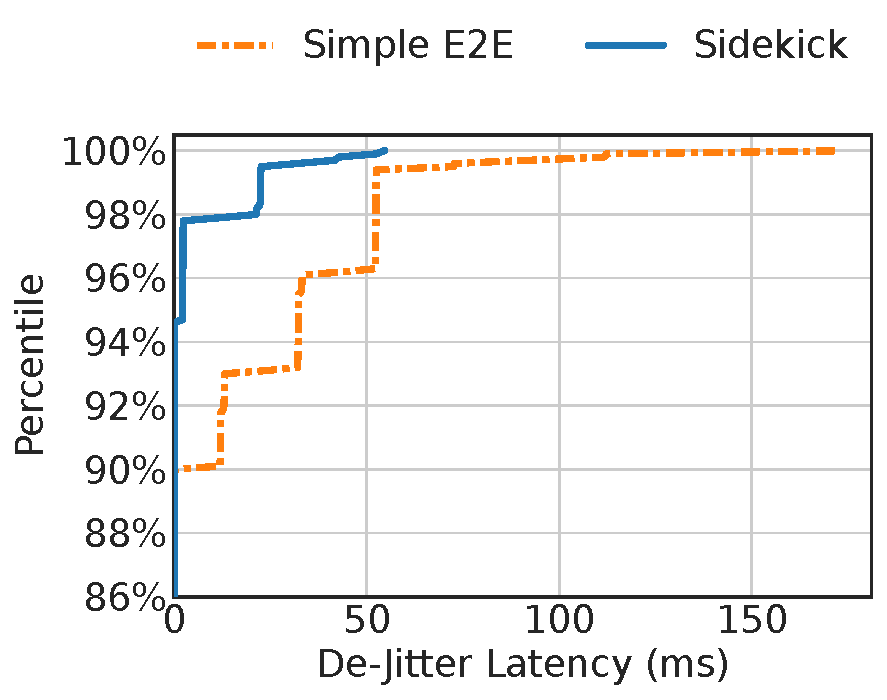
\includegraphics[width=\linewidth]{sidekick/figures/fig4a_low_latency_media.pdf}
\caption{Scenario \#1:
 Reduced tail latency of de-jitter delay
with earlier retransmission in the low-latency media application. 5 minute trials.}
\label{fig:sidekick:main-results:media}
\end{subfigure}
\hfill
\begin{subfigure}{0.31\textwidth}
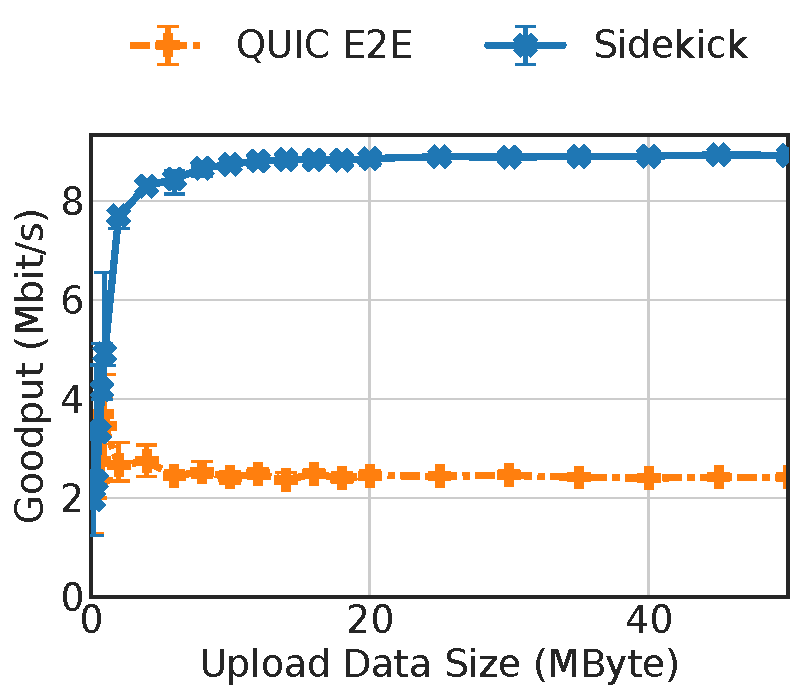
\includegraphics[width=0.97\linewidth]{sidekick/figures/fig4b_pep_emulation.pdf}
\caption{Scenario \#2: Improved goodput in the connection-splitting PEP emulation.
Error bars are the IQR of 20 trials.
}
\label{fig:sidekick:main-results:pep-emulation}
\end{subfigure}
\hfill
\begin{subfigure}{0.32\textwidth}
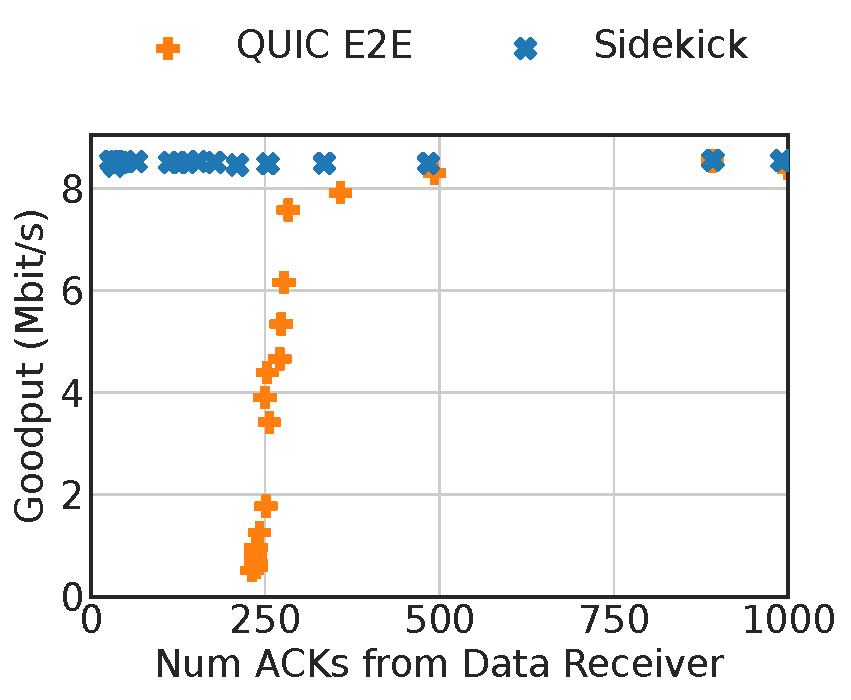
\includegraphics[width=0.99\linewidth]{sidekick/figures/fig4c_ack_reduction.pdf}
\caption{Scenario \#3:
High goodput independent of end-to-end ACK frequency in the ACK reduction scenario.
10 MB upload.}
\label{fig:sidekick:main-results:ack-reduction}
\end{subfigure}
\caption{
Comparing the end-to-end baseline protocol to the same protocol with a Sidekick
connection, using the success metrics for the three scenarios described in
\Cref{tab:sidekick:experimental-scenarios}.
}
% \dm{Maybe a notation like $x/4$ would be more suggestive than $4x$?}
\label{fig:sidekick:main-results}
\end{figure*}
